\chapter{Dataset}\label{chapter-dataset} 

This part of the thesis provides a brief overview of what pulsar stars are. It then goes on to explain the two modes of the dataset used for their detection: the integrated profile (IP) and dispersion measure (DM). The most part of this chapter is a direct summary of the background chapter in the doctoral thesis \citep{lyon}\footnote{\citep{lyon} can be accessed \href{http://www.scienceguyrob.com/wp-content/uploads/2016/12/WhyArePulsarsHardToFind_Lyon_2016.pdf}{here}} . Some parts of the text are barely changed from \citep{lyon}, nevertheless, many details have been voluntary ignored for the sake of simplicity as it is not the focus of this work. 

A star is a luminous ball of gas, mostly hydrogen and helium, held together by its own gravity. The nearest star of Earth is the Sun. Most mass is in the core, at the center of the star. Gravitational forces are by consequence directed inwards. During the majority of a star's life, it will fuse hydrogen to helium, generating an outwards pressure, balancing the gravity \citep{ghosh}. By the time the hydrogen amounts become insufficient, the star starts to use other elements in the surrounding layers of the core as a fuel. As those elements diminish, the star's energy output drops rapidly, causing gravity to overcome the forces which had previously maintained the stars structure. The core of the star than undergoes a rapid and violent collapse \citep{ghosh}. The collapse can lead to a number of potential evolutionary outcomes for the leftover core (see Figure \ref{fig:evol-endpoints}), depending on the stars birth mass measured in solar masses ($M_{\bigodot}$). Intuitively, the heavier the birth mass, the greater the inwards gravitational force are and the harder the collapse. The first outcome applies to low mass stars, which typically become white dwarfs following their collapse. Within white dwarfs, densely packed electrons are able to resist gravitational compression. Our own sun is likely to one day become a white dwarf star. Then there are stars between 8-20 $M_{\bigodot}$ at birth, electron degeneracy pressure can no longer prevent collapse as in white dwarfs, but they are not massive enough to undergo complete gravitational collapse, preventing the formation of a black hole. Instead the intense conditions within these stars cause electrons to combine with protons forming neutrons who resist against pressure; These stars are called neutron stars. The last evolutionary outcome applies to large stars with masses greater than 20 $M_{\bigodot}$. These stars can, under the right conditions, undergo complete gravitational collapse. This results in the formation of a black hole singularity otherwise known as a stellar mass black hole. 
\begin{figure}[!ht]
\centering
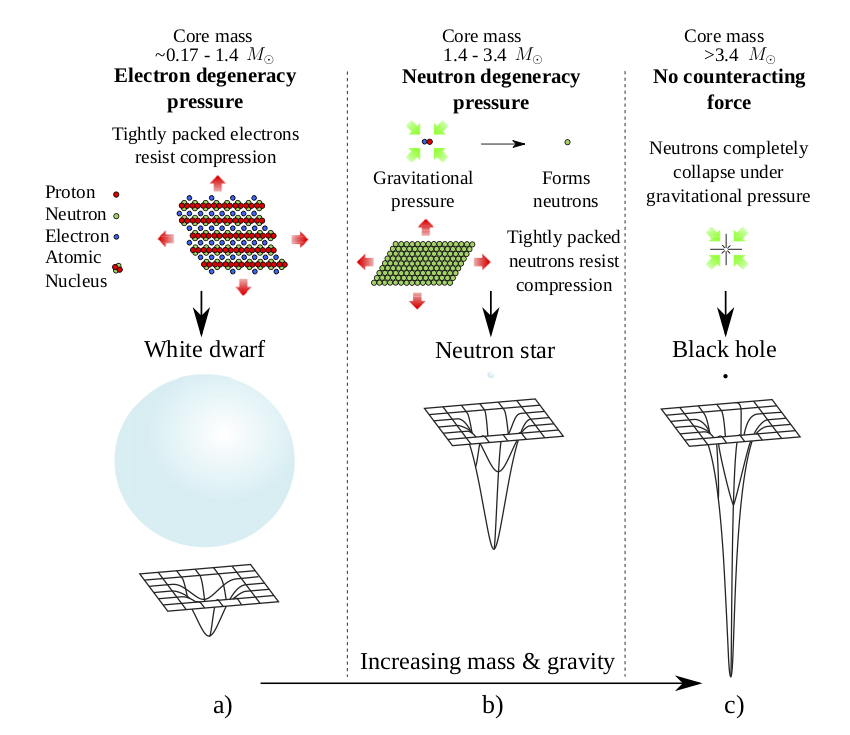
\includegraphics[scale=0.4]{figures/screenshot-1}
\caption[Evolutionary endpoints for main sequence stars]{Common evolutionary endpoints for main sequence stars. In a) electron degeneracy pressure prevents gravitational collapse, leading to the formation of a white dwarf star. In b) electron degeneracy pressure is no longer enough to counteract the inward force of gravity, however the gravitational pressure is insufficient to overcome neutron degeneracy pressure, allowing a Neutron star to form. Finally in c) the force of gravity is so great that gravitational collapse cannot be halted, resulting in the formation of a black hole. The depictions of the gravitational sinks above are based on diagrams by \citep{star-eater}. \textit{Image and caption copied from} \citep{lyon}.}	
\label{fig:evol-endpoints}
\end{figure}

A pulsar is a unique form of neutron star that retained most of its angular momentum of their progenitor star during collapse. Complex interactions between the surfaces of pulsars and their strong magnetic fields, helps to produce their defining feature, the emission of radio waves. The radio emission produced by pulsars originates from their magnetospheres \citep{ghosh}. This is the area of space surrounding a pulsar in which charged particles are influenced by a co-rotating magnetic field, which has both open and closed field lines \citep{lorimer} (see Figure \ref{fig:fig-1}). To maintain this co-rotation property, the velocity of the field lines must increase as they move further away from the pulsar. Eventually the distance becomes so great, that to maintain co-rotation, the velocity of the field lines must be greater than or equal to the speed of light $c$. This is not possible, thus the field lines are unable to close where the required velocity is $c$. The abstract cylinder aligned with the rotation axis, that synchronously rotates with the pulsar at a velocity $c$, is known as the light cylinder (see Figure \ref{fig:fig-1}). The particles extracted from the surface are then believed to be accelerated along the co-rotating magnetic field lines of the magnetosphere \citep{lorimer2008}, which endows the particles with increased energy. This additional energy causes the particles to emit radiation \citep{lorimer2008} to be emitted along the open field lines near a pulsar's magnetic pole. A pulsar's magnetic axis is usually inclined with respect to its rotational axis. Therefore each time a pulsar rotates, the radiation beam produced near the magnetic poles, is swept at an angle across the sky. If the beam crosses the line of sight of an observer here on Earth, the pulsar becomes detectable as a rise and fall in broadband radio emission. This pattern repeats periodically with each rotation of the pulsar. This is known as the lighthouse model of emission \citep{lorimer2008}, because the beam of radiation is analogous to a lighthouse warning light rotating very quickly.
\begin{figure}[!ht]
\centering
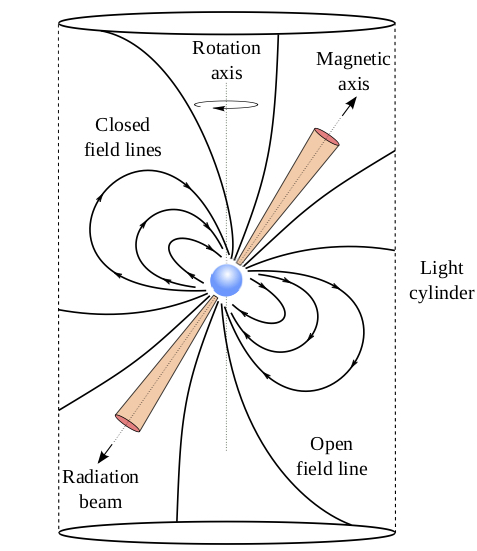
\includegraphics[scale=0.4]{figures/fig-1}
\caption[Lighthouse model of a radio pulsar]{Simplification of the lighthouse model of a radio pulsar, the pulsar is surrounded by a strong magnetic field comprising of open and closed field lines unable to close at the light cylinder. The light cylinder is an imaginary cylinder aligned with the pulsars rotational axis, that synchronously rotates with the pulsar at the speed of light. As the magnetic field cannot rotate at this velocity, the field lines cannot close at the light cylinder leading to open field lines. Radio pulses are emitted from the open field lines at a region near the magnetic poles in the pulsar’s magnetosphere. \textit{Image and caption copied from} \citep{lyon}.}	
\label{fig:fig-1}
\end{figure}

Each pulsar produces a unique pattern of pulse emission known as its pulse profile \citep{lorimer2008}. Two such profiles are shown in Figure \ref{fig:fig-3}. However whilst pulsar rotational periods are extremely consistent, their profiles can deviate from one-period to the next. Whilst such changes in the pulse profile provide clues to what is happening in and around the pulsar, they make pulsars hard to detect. This is because their signals are non-uniform and not entirely stable overtime. However these profiles do become stable, when averaged over many thousands of rotations.
\begin{figure}[!h]
\centering
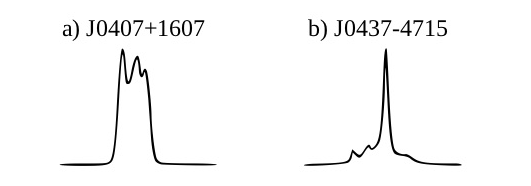
\includegraphics[scale=0.4]{figures/fig-3}
\caption[Pulse profiles of two separate pulsars]{Example pulse profiles of two separate pulsars. These profiles were adapted from those originally presented in \citep{lorimer}.  \textit{Image and caption copied from} \citep{lyon}.}	
\label{fig:fig-3}
\end{figure}

Signals travelling through the interstellar medium (ISM) are affected, the most significant effect is known as dispersion. As pulsar signals travel through the ISM towards the Earth, they interact with charged particles (free electrons) on route. These interactions delay the arrival of the signal here on Earth. The low frequency components of the signal are delayed more than the corresponding high frequency counterparts. This has a dispersive effect that causes pulsar signals to become smeared in time. This makes it difficult to detect pulsars, as their pulses become less pronounced as shown in Figure \ref{fig:fig-4}. Manifesting itself as a reduction in the signal-to-noise ratio of a detected pulse. The amount of dispersive smearing a signal receives is proportional to a quantity called the dispersion measure (DM) \citep{lorimer}. The DM is the integrated column density of free electrons between an observer and a pulsar \citep{lorimer2008}. The true column density, and thus the precise degree to which a signal is dispersed, cannot be known a priori. A number of dispersion measure tests or "DM trials", must therefore be conducted to determine this value as accurately as possible. An accurate DM can be used to undo the dispersive smearing, allowing the signal-to-noise ratio of a detected signal to be maximised \citep{lorimer}. For a single dispersion trial, each frequency channel is shifted by an appropriate delay. Subsequent trials increment the delay in steps, until a maximum DM is reached. This maximum will vary according to the region of sky being surveyed, the observing frequency, and bandwidth. The process produces one 'de-dispersed' time series per frequency channel. These are then summed to produce a single de-dispersed time series per trial (as shown at the bottom plot of Figure \ref{fig:fig-4} a). In total de-dispersion produces a number of time series equal to the total number of DM trials.
\begin{figure}[!h]
\centering
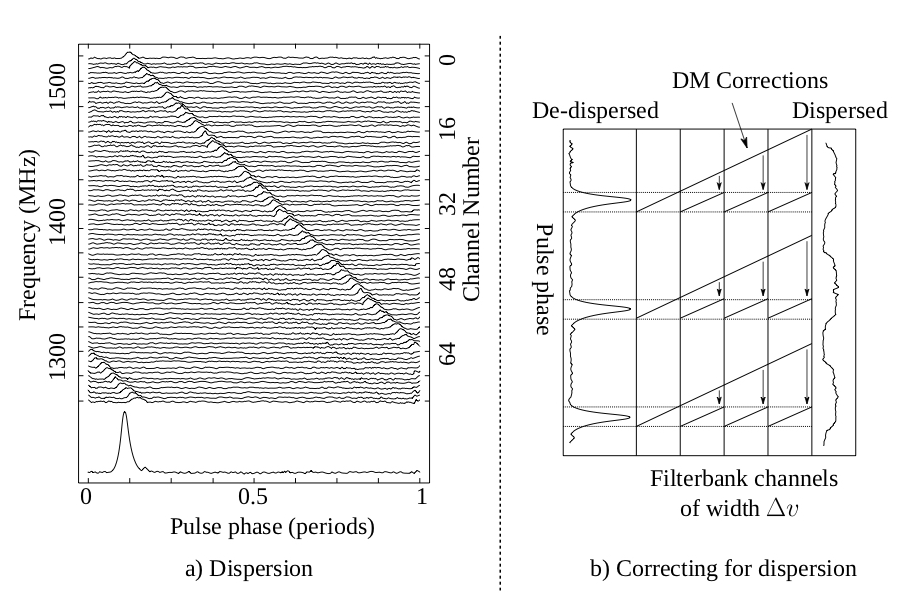
\includegraphics[scale=0.3]{figures/fig-4}
\caption[Signal Dispersion]{An example of signal dispersion. Based upon diagrams originally presented in \citep{lorimer}. Plot a) shows how a signal is dispersed in time. Dispersion hides the true pulse shape and causes a lowering of the detected signal-to-noise. Plot b) shows the application of DM corrections to a dispersed signal. The DM correction is different in each frequency channel, since dispersion is proportional to frequency. \textit{Image and caption copied from} \citep{lyon}.}	
\label{fig:fig-4}
\end{figure}

By precisely measuring the timing of such pulses, astronomers can use pulsars for unique experiments at the frontiers of modern physics. Indeed, pulsars exist in strong-field gravitational environments due to their enormous mass. It is impossible to study such environments within Earth-based laboratories, or even within the confines of our own solar system which is lightweight by comparison. In the strong-field environment provided by pulsars, their immense gravitational fields directly affect the arrival times on Earth of the signals they produce, via special and general-relativistic effects. By studying these effects, tests of many gravitational theories can be accomplished.  Another application of measuring the arrival time of pulses is that they are effective time keeping system, rivalling atomic clocks for accuracy. Such clocks are useful for spacecraft navigation and timekeeping here on Earth.